
\documentclass[10pt]{article}

\usepackage{pgfplots}
\usepackage{tikz}
\usepackage{amsmath}
\usepackage{amssymb}     % for mathbb
\usepackage{enumerate}
\usepackage{xfrac}
\usepackage{float}
\usepackage{hyperref}
\usepackage{algorithmic}
\usepackage{algorithm}
\usepackage{booktabs}    % for beautiful tables
\usepackage{array}    
\usepackage{multirow}
\usepackage{siunitx}     % for si units
\usepackage{color}
\usepackage{titlesec}    % for header spacing
\usepackage{caption}     % for caption*
\usepackage[capitalize]{cleveref}

\usepackage[backend=bibtex,style=ieee]{biblatex}

% set margins
\addtolength{\oddsidemargin}{-.875in}
\addtolength{\evensidemargin}{-.875in}
\addtolength{\textwidth}{1.75in}
\addtolength{\topmargin}{-.875in}
\addtolength{\textheight}{1.75in}

\setlength{\parindent}{0cm}        % no paragraph indentations
\setlength{\parskip}{0.5em}        % small paragraph spacing

\titlespacing\section{0pt}{10pt plus 4pt minus 2pt}{0pt plus 2pt minus 2pt}
\titlespacing\subsection{0pt}{10pt plus 4pt minus 2pt}{0pt plus 2pt minus 2pt}
\titlespacing\subsubsection{0pt}{10pt plus 4pt minus 2pt}{0pt plus 2pt minus 2pt}

\DeclareMathOperator*{\argmax}{arg\,max}

\newcommand\MyBox[1]{
  \fbox{\lower0.75cm
    \vbox to 1.7cm{\vfil
      \hbox to 1.7cm{\hfil\parbox{1.4cm}{#1}\hfil}
      \vfil}%
  }%
}

\newcommand{\calcium}[0]{Ca\textsuperscript{2+}}
\newcommand{\todo}[1]{\textcolor{red}{#1}}
\providecommand{\tw}[1]{{\tw[TIM: #1]}}

% monokai colors
\definecolor{color1}{RGB}{82,227,246}  % light blue
\definecolor{color2}{RGB}{167,243,113} % light green
\definecolor{color3}{RGB}{255,0,127}   % red
\definecolor{color4}{RGB}{249,151,31}  % orange
\definecolor{color5}{RGB}{121,171,255} % cobalt

\AtEveryBibitem{
\ifentrytype{inproceedings}{
    \clearlist{address}
    \clearlist{publisher}
    \clearname{editor}
    \clearlist{organization}
    \clearfield{url}  
    \clearfield{doi}  
    \clearfield{pages}  
    \clearlist{location}
 }{}
 }

\addbibresource{ref.bib}
\renewcommand*{\bibfont}{\footnotesize}

\begin{document}

\begin{center}
    {\LARGE Clustering of Neurons from Large-Scale Calcium Imaging Data}

    Stats 306b Project - Final Report

    Mohammad Ebrahimi and Tim Wheeler

    Spring 2015
\end{center}

\begin{abstract}
Fluorescent imaging allows for the analysis of signalling behavior on a per-neuron basis in anesthetized and awake behaving animals. % ~\cite{Mukamel2009}
Existing methods monitor {\calcium} dynamics over a large region, but recently developed automated methods allow for isolating signals and associating them with particular neurons.
The resulting set of candidate neurons suffers from the presence of background structures such as blood vessels.
This project applies clustering methods to candidate objects in a one-photon {\calcium} dataset for the classification of neurons from background structures.
\todo{Hierarchical clustering was performed to identify preliminary classes.}
\todo{Principle component analysis was performed to identify preliminary important features and a clustering analysis was conducted using the first two principle components.}
\todo{Sparse clustering and sparse principle component analysis were conducted to identify a reduced featureset which captures the majority of the variation in the data.}
\todo{Group validation was performed by comparing the clusters obtained in the first dataset to the clusters obtained in a withheld dataset.}
\todo{Results indicate...}
\end{abstract}


\section{Introduction}

A fundamental objective for neuroscience is understanding the relationship between neuron activity and resulting high level behavior.
Recent studies have sought to use recorded neuronal activity in live animals performing various tasks in order to obtain correlations between individual neurons or groups of neurons to the animal's behavior. Fluorescence microscopy is one recording method which picks up fluorescent markers given off by neurons in the brain, modulated by their ``firing'', and allows for the simultaneous imaging of large cranial regions.

The work presented in this paper is based on data obtained by the Schnitzer group which collected neuron activity in freely-behaving mice and rats~\cite{Ghosh2011}. 
A fluorescent microscope surgically attached to the skull collects data as the animal wanders about its environment.
This results in a video recording of a \num{500} $\mu$m $\times$ \num{500} $\mu$m section of the primary visual cortex.


Previous work by \citeauthor{Mukamel2009} obtained one-photon {\calcium} imaging recordings from the primary visual cortex of awake behaving mice.
Their work isolated candidate objects from cortex recordings of mice performing a go/no-go task for \num{30}-minute sessions over three consecutive days.
They demonstrated a novel method which leveraged spatio-temporal sparseness in elevated [\calcium] levels to identify neuronal spikes and associate them with particular regions in the source frames.
The resulting set of candidate neurons includes background structures such as blood vessels alongside actual neurons.
This project aims to apply unsupervised learning methods to automatically classify neurons from background structure.

Several forms of analysis are applied to the dataset.
First, an extensive set of features were extracted from both each candidate object's signal trace and averaged calcium image.
Second, full and sparse hierarchical clustering were performed to identify preliminary neuronal classes.
The importance of various features were compared and suitable clusters were identified.
Finally, group validation was performed by comparing the clusters obtained in the first dataset to the clusters obtained in a withheld dataset.

\section{Data Source}


This work uses the isolated candidate objects, including frame images assocated with each of the extracted independent components and averaged signal traces associated with each candidate.

The complete cortex recording was segmented into a four-by-four grid.
Candidate object images are \num{500} $\times$ \num{500} pixel black and white frame averages that show the strength of their respective independent component over its corresponding segmented field of view. 
The pixel values correspond to the flourescent signal of the identified object, which may be a neuron, part of a blood vessel, or background noise.

Independent component traces were sampled at \num{6.7}\si{Hz}, totalling \num{1200} samples over each \num{30}-minute recording. The component traces of neurons possess indicative spikes with tapered decays corresponding to neuron activity, but also contain significant background noise.

Each recording contains a few thousand extracted objects, the idendity and quantity of which will vary between recordings.
The final feature set includes \num{5450} samples.

Each candidate object was hand-labelled as either a neuron or background structure. 
According to this labelling approximately \num{50}\% of the candidate objects are actual neurons.
While this labelling does provide a measure of ground-truth it is still subjective and could contain incorrect classifications.

\section{Features}

A set of \num{42} candidate features was extracted from the segmented image data and associated intracellular [\calcium] signals as is listed in~\cref{table:allfeatures} in the Appendix.
The set includes \emph{image features} obtained from the grayscale frame averages and \emph{trace features} from the independent component time series traces.

\subsection{Image Features}

\begin{figure}[h]
    \centering
    \begin{minipage}{.33\textwidth}
      \centering
      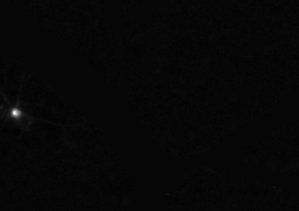
\includegraphics[width=.9\linewidth]{figs/frame_2.png}
      \caption*{\footnotesize A) Clean neuron source frame.}
      \label{fig:frame1}
    \end{minipage}%
    \begin{minipage}{.33\textwidth}
      \centering
      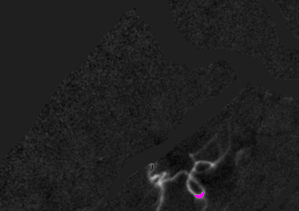
\includegraphics[width=.9\linewidth]{figs/frame_3.png}
      \caption*{\footnotesize B) Background structure. }
      \label{fig:frame2}
    \end{minipage}
    \begin{minipage}{.33\textwidth}
      \centering
      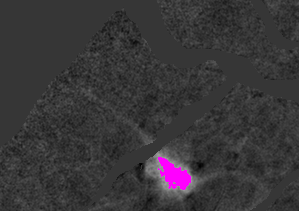
\includegraphics[width=.9\linewidth]{figs/frame_4.png}
      \caption*{\footnotesize C) Large neuron. }
      \label{fig:frame3}
    \end{minipage}
    \caption{\footnotesize Examples of frame data. (A) contains a clean neuron source frame. (B) contains background structure in the form of blood vessels. The FWHM peak region is colored magenta. (C) contains an unknown structure which is likely a neuron. Here the peak region is much larger. }
\end{figure}

A set of twelve features were extracted for each image frame.
A frame is a \num{500} by \num{500} pixel monochromatic matrix containing the average IC over the segemented field of view. 
Image frame values background noise fluctuates on the order of \num{+-3} but contains sharp peak values as high as \num{100} in intensity.

A single peak region was identified in each image using the full-width half maximum.
All pixels above half the maximum value were considered, and a flood-fill algorithm was used to find the largest connected region, hereafter referred to as the peak region.

Several features are derived directly from the peak region.
The \emph{peak region size} is the number of pixels in the peak region, and corresponds roughly to the area of the peak region.
The \emph{peak region perimeter} is the number of pixels on the exterior of the peak region, and corresponds roughly to the perimeter of the peak region.
An approximate measure of \emph{roundness} was obtained by computing the ratio of the peak region size and perimeter, $\text{roundness} = 4\pi \sfrac{\text{area}}{\text{perimeter}^2}$, 
where a roundness of one corresponds roughly to a perfect circle.
The peak region \emph{skew} was obtained by computing the $xy$-correlation between the square subsection of the image of twenty-one pixel side length centered at the peak region center.
The \emph{peak} value of the peak region was extracted, as well as the peak region \emph{mean} and \emph{standard deviation}.

A subimage of twenty-four pixel side length was extracted about the peak region center and used to compute additional features, among them the mean and standard deviation of the subimage.
A measure of \emph{contrast} and \emph{directionality} was obtained using the Tamura definition~\cite{Tamura1978}.
Contrast is a measure of image sharpness, and was calculated using

$$
F_\text{con} = \frac{\sigma}{\alpha_4^z} \quad \text{with} \quad \alpha_4 = \frac{\mu_4}{\sigma^4}
$$

\noindent
where $\mu_4 = \frac{1}{nm} \sum_{i=1}^n \sum_{j=1}^m (IC(i,j)-\mu)^4$
is the fourth moment about the mean $\mu$, $z$ is \num{0.25} from experiment, and $\sigma^2$ is the variance of the image values.

Directionality was computed using the approximate horizontal and vertical derivatives from convolution with the following $3\times3$ matrices, respectively $\Delta_V$ and $\Delta_H$:

$$
\begin{bmatrix}
-1 & 0 & 1 \\ -1 & 0 & 1 \\ -1 & 0 & 1
\end{bmatrix} \qquad
\begin{bmatrix}
-1 & -1 & -1 \\
0 & 0 & 0 \\
1 & 1 & 1
\end{bmatrix}
$$

\noindent
and then computing $\theta = \frac{\pi}{2} + \tan^{-1}\frac{\Delta_V(i,j)}{\Delta_H(i,j)}$ for each pixel in the image.
These values were discretized into a sixteen bin histogram.

Some peak images are very close to their segmented image borders. For these images it is not possible to extract the subimage.
The corresponding features were imputed using the method of iterated singular value decomposition of rank \num{10}.

\subsection{Trace Features}

Calcium activity for a perfectly recorded neuron takes the form of temporally sparse spikes that start with a fast jump followed by exponential decay. Spike sparsity and exponential decay constants vary between neurons~\cite{Mukamel2009}. 
An example trace is shown in \cref{fig:trace}.

For each trace a \emph{high threshold} and \emph{low threshold} were calculated where the \emph{CDF} used is \todo{\num{0.97}} and \todo{\num{0.03}} respectively. In addition, every time the trace crosses the high threshold and low threshold line, a high crossing and low crossing event is detected. These events can be described by a \emph{rise time}, \emph{fall time} and \emph{pick value}. The mean and variance of these three variables were also computed. The \emph{ratio of mean pick value to threshold value} of high or low crossings were also extraced.

The sparsity of neural activity has been previously shown to be a good indicator~\cite{Kim2011}. Average and variance of \emph{crossing event intervals} for high and low crossings were taken where each interval is the time distance between two picks of the crossing events.  The ratio of \emph{total crossing duration} to the total time were calculated for each family separately and taken as a sparsity measure. Neurons are expected to have primarily high crossing events. The \emph{number of high crossing events}, \emph{number of low crossing events} and the ratio of these two were also included. The final trace feature vector includes \num{30} indices.

\begin{figure}[h]
    \centering

    \begin{minipage}{1\textwidth}
      \centering
      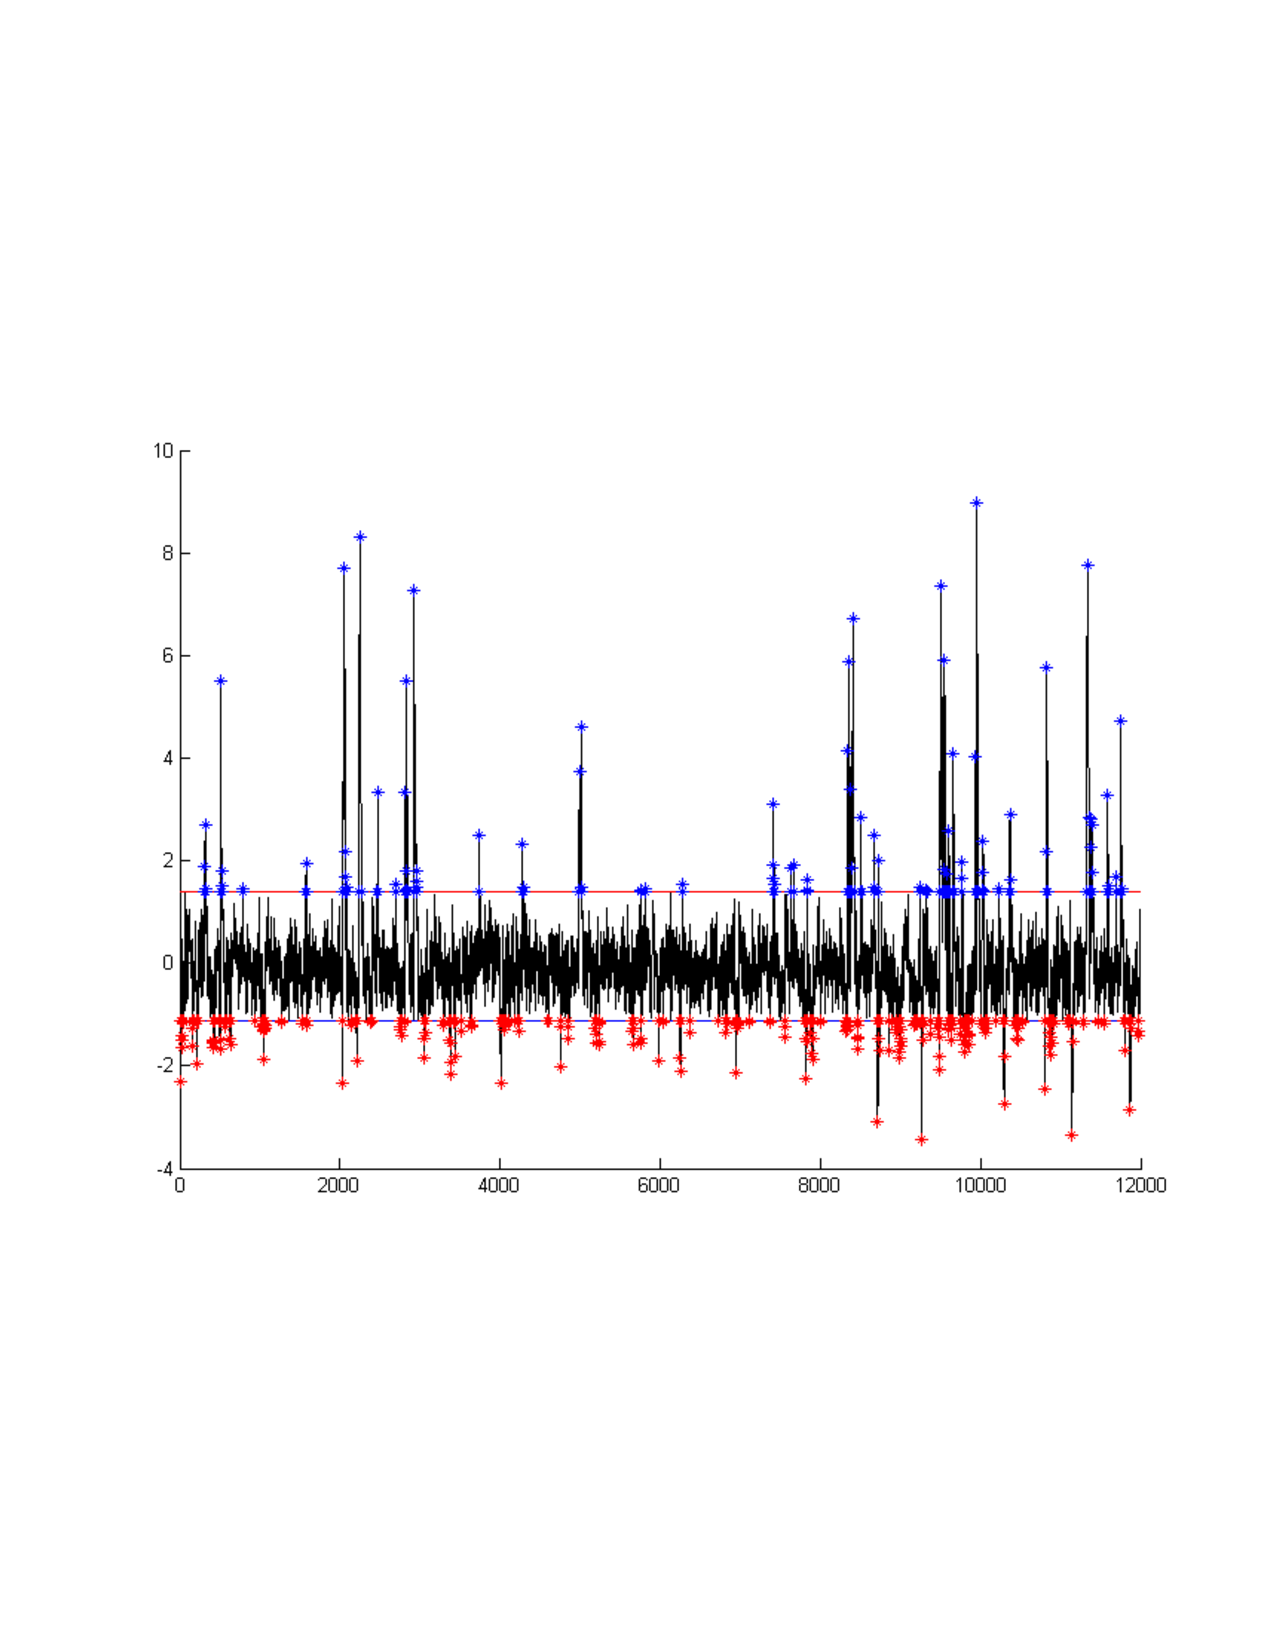
\includegraphics[width=0.4\linewidth]{figs/trace.pdf}
      \caption{\footnotesize Example neuron Calcium trace. \textcolor{blue}{blue *} indicates start, pick and end of high crossing events and \textcolor{red}{red *} indicates the same values for low crossing events }
      \label{fig:trace}
    \end{minipage}
\end{figure}

\section{Analysis}

The objective of this analysis was to identify clusters within the calcium imaging dataset which correspond to neurons and background structure, respectively. During the process it may be possible to further identify subclusters which correspond to different types of neurons or types of background structure.

Hierarchical clustering possesses several advantages over partitional clustering for this problem.
First, most of the features in the dataset are continuous and poorly separated, making it difficult for a partitional algorithm such as $k$-means to accurately divide it by a hard boundary. 
Secondly, hierarchical clustering produces dendrograms, which contain a full range of clusters, allowing for the appropriate cutoff point to be chosen by a statistician via inspection. 
Third, hierarchical clustering is deterministic and does not require specifying the number of desired clusters ahead of time.

The dataset was subjected to several forms of hierarchical clustering in an effort to identify suitable neuronal clusters and identify the most important features. 
All analysis used a data matrix in which each feature vector was de-meaned and divided by its standard deviation.
A final round of analysis was performed to validate the obtained clusters against a second withheld dataset.

\subsection{Full Hierarchical Clustering}

Agglomerative clustering using complete linking and Euclidean distance was conducted and the results are shown in \cref{fig:fullhierarchical}.
Six well-separated clusters were extraced from the dendrogram, four neuronal clusters and two corresponding to background structure.

\begin{figure}[h]
    \centering

    \hspace{-1cm}
    \begin{minipage}{0.6\textwidth}
      \centering
      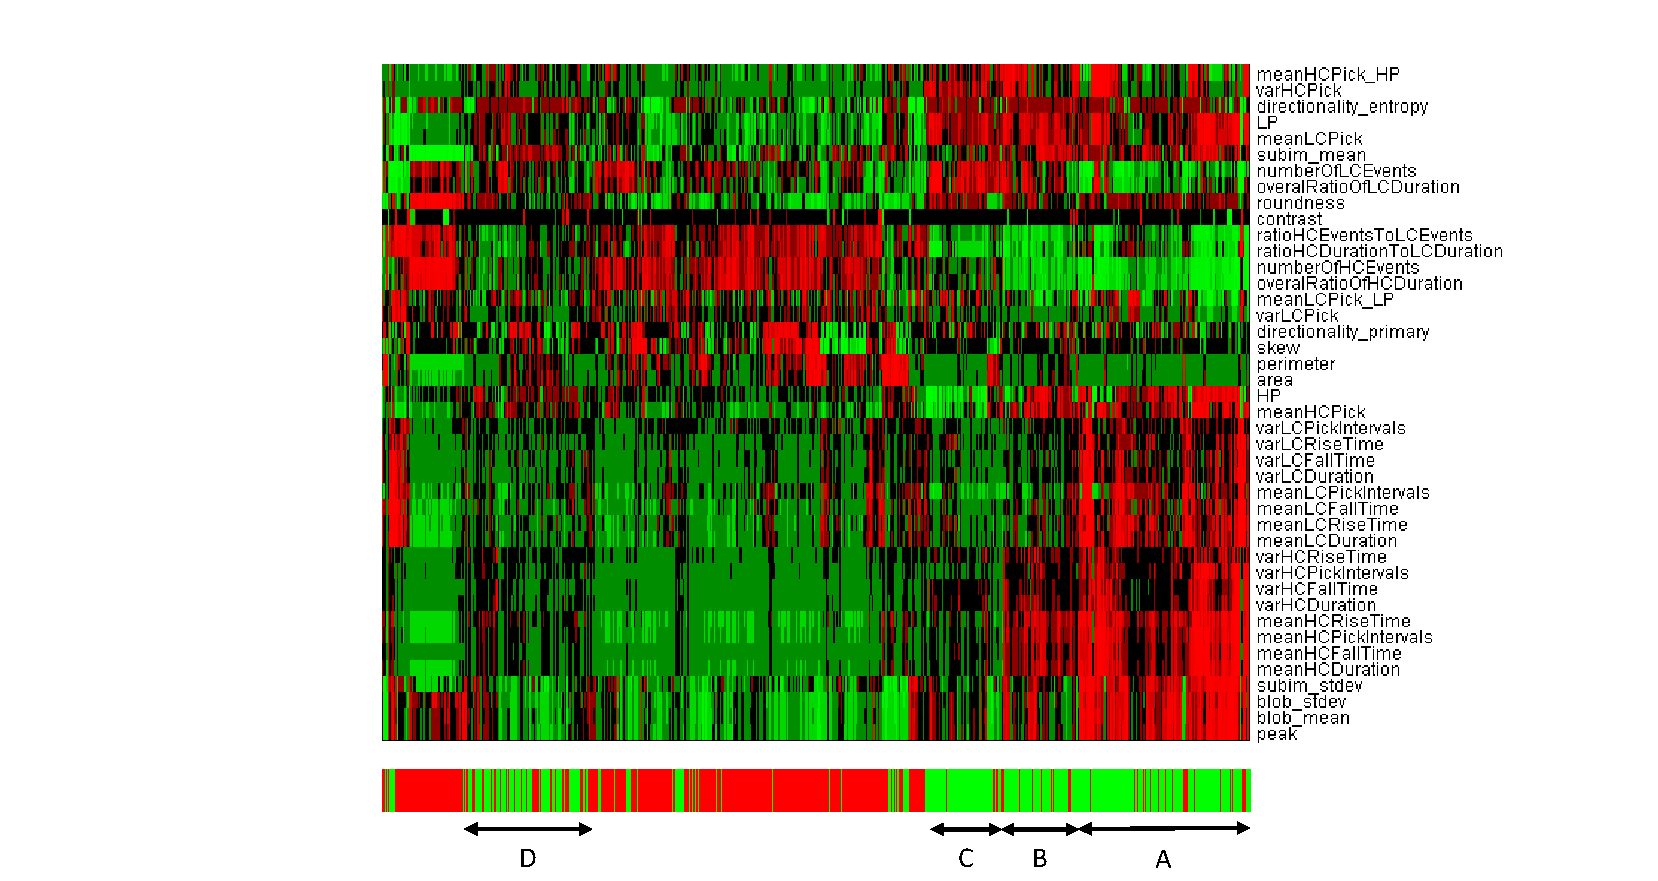
\includegraphics[width=\textwidth]{figs/fig7_cropped.pdf}
    \end{minipage}
    \hspace{-1cm}
    \begin{minipage}{0.45\textwidth}
      \centering
      \footnotesize
      \begin{tabular}{cSS}
        \toprule
        Cluster & {Size} & {Percent Neurons (\%)} \\
        \midrule
        A & 1070 & 88.3 \\
        B &  496 & 88.9 \\
        C &  428 & 90.2 \\
        D &  838 & 66.5 \\
        High Intensity & 2121 & 14.8 \\
        Low Intensity &  497 &  6.8 \\
        \bottomrule
      \end{tabular}
    \end{minipage}
    \caption{\footnotesize Full hierarchical clustering and associated cluster statistics.}
    \label{fig:fullhierarchical}
\end{figure}

Four clusters of high neuron content were identified, three of which contain approximately \num{90}\% neurons and a fourth containing \num{66.5}\%. Together, these four clusters account for \num{87}
\% of all cells in the dataset.

The extracted clusters appear to be group according to the depth and the layer of the soma from which the neuron is located. 
Figure \cref{fig:clusterdepths} in the Appendix shows the aggregated image constructed for each cluster across the entire imaged region. 
The image of cluster A is well focused wheras the images for clusters B through D become less focused. 

In addition to the two neuron clusters, two clusters for background structure were identified. The first corresponds to highly visible vesseles whereas the second contains low-intensity background material. These are shown in \cref{fig:clusterdepths} in the appendix.


\subsection{Principle Component Analysis}

Further insight into the relative importance of features in clustering was obtained by investigating the principle components.
The first two principle components capture \num{23.6}\% of the variation in the data.
The original feature space is moderately uncorrelated.
Capturing \num{90}\% of the variation requires using the first \num{23} out of \num{42} principle components.
The variation curve is shown in \cref{fig:variation} along with a scatter plot of the ground-truth classification.

\begin{figure}[h]
    \centering

    \begin{minipage}{0.25\textwidth}
      \centering
      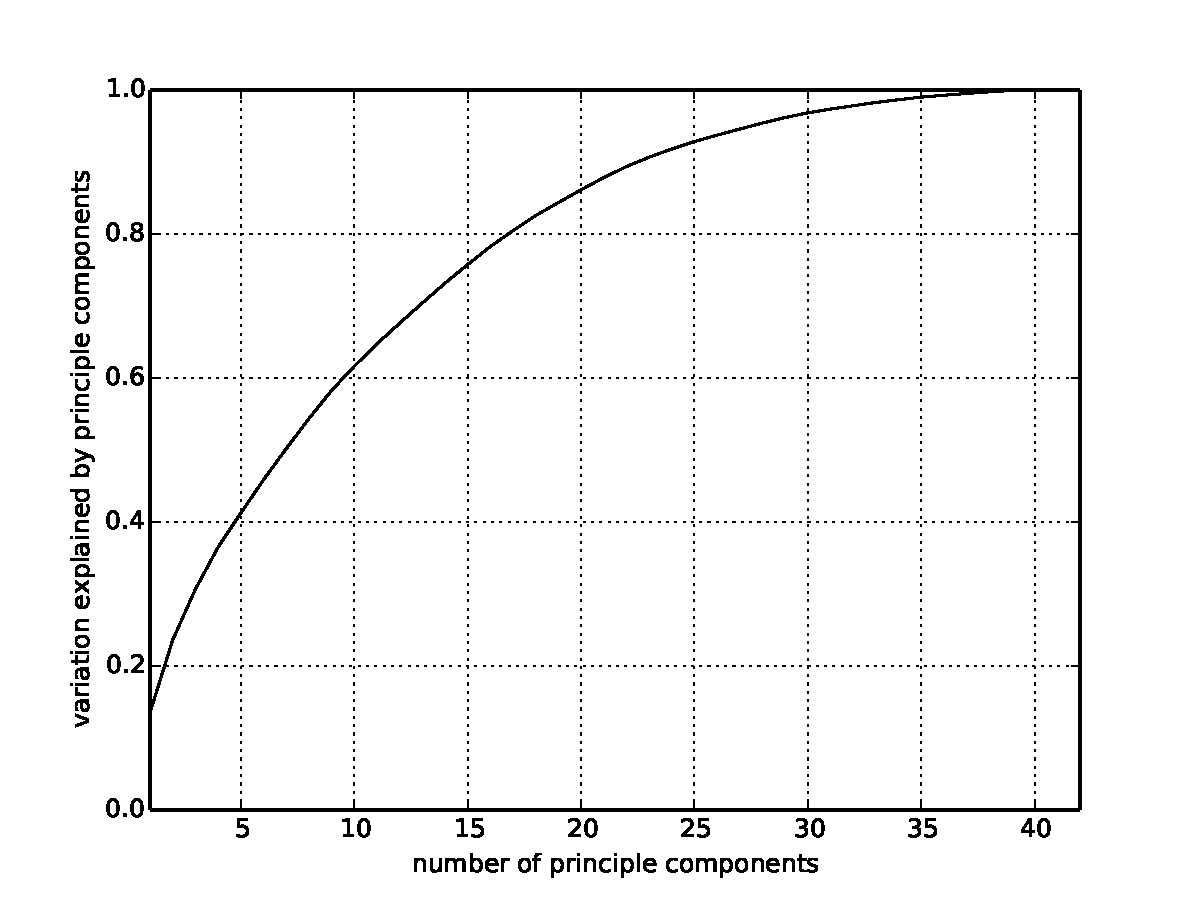
\includegraphics[width=\textwidth]{figs/variation.pdf}
    \end{minipage}
    \begin{minipage}{0.70\textwidth}
      \centering
      \vspace{2mm}
      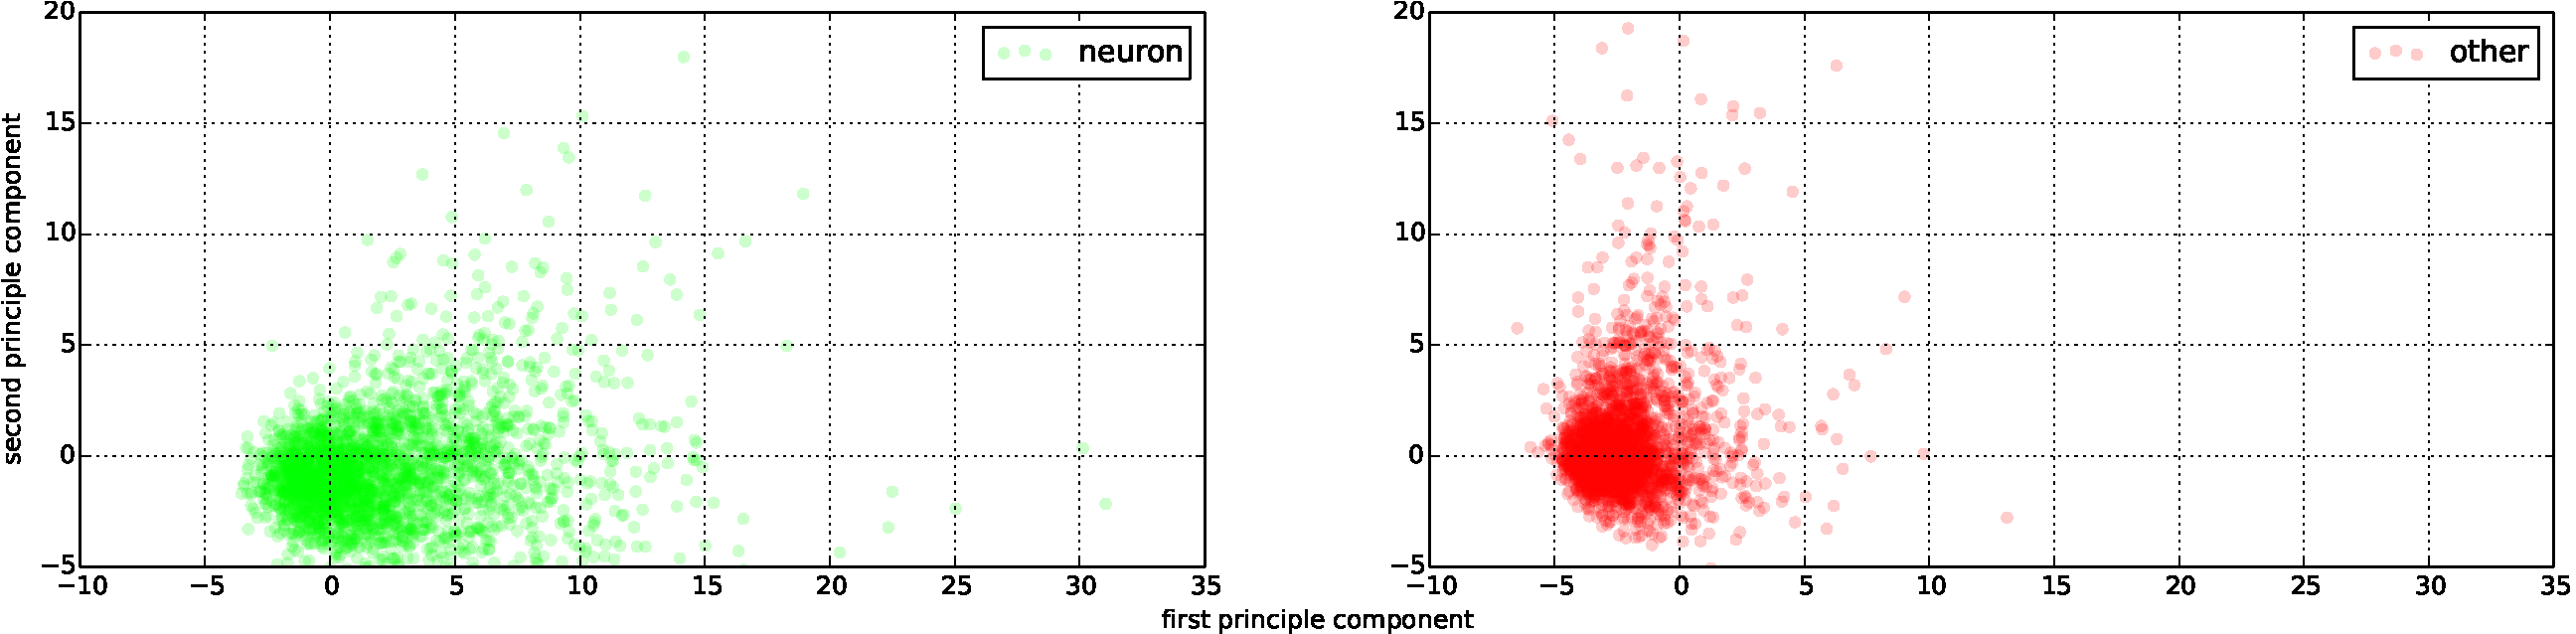
\includegraphics[width=\textwidth]{figs/PCA_scatter_cropped.pdf}
    \end{minipage}
    \caption{\footnotesize The variation curve and Ground truth scatter along first two principle components}
    \label{fig:variation}
\end{figure}

A scatter plot of the matching matrix classes along with the corresponding confusion matrix are given in \cref{fig:confusion}. The scatter plot clearly shows how the majority of incorrect labels occur in the overlapping region between labels. The clusters obtain an accuracy of \num{0.844} and a precision of \num{0.870}. Note that the ground truth class labels are based on human judgement and could contain several incorrect labels.

\begin{figure}[h]
    \centering

    \begin{minipage}{0.5\textwidth}
      \centering
      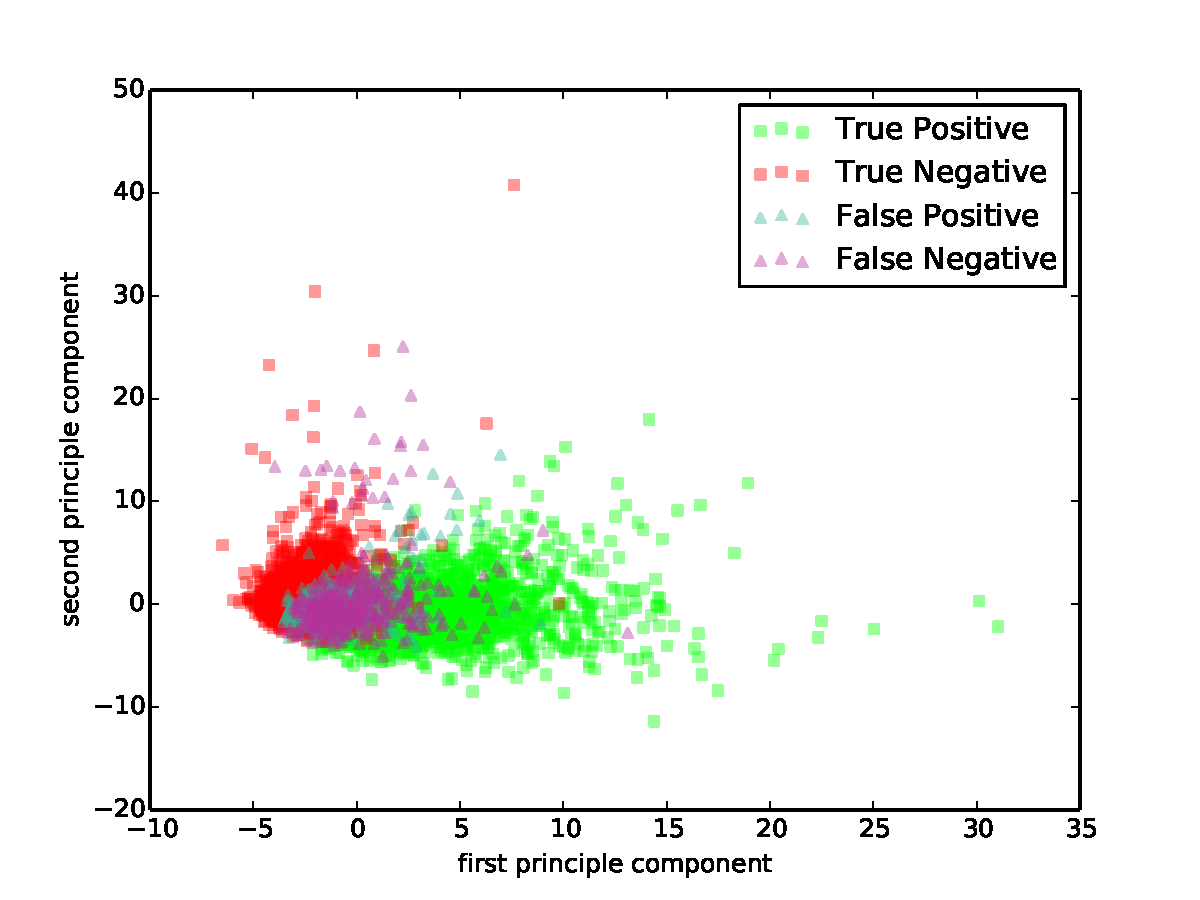
\includegraphics[width=0.8\textwidth]{figs/PCA_confusion.pdf}
    \end{minipage}
    \begin{minipage}{0.45\textwidth}
      \centering
      \scriptsize

        \renewcommand\arraystretch{1.5}
        \setlength\tabcolsep{0pt}
        \begin{tabular}{c >{\bfseries}r @{\hspace{0.7em}}c @{\hspace{0.4em}}c @{\hspace{0.7em}}l}
          \multirow{10}{*}{\parbox{1.1cm}{\bfseries\raggedleft Actual\\ Value}} & 
            & \multicolumn{2}{c}{\bfseries Predicted Outcome} & \\
          & & \bfseries p & \bfseries n & \bfseries total \\
          & p$'$ & \MyBox{\num{2329}} & \MyBox{\num{503}}  & \num{2832} \\[2.4em]
          \addlinespace[0.3em]
          & n$'$ & \MyBox{\num{347}} &  \MyBox{\num{2271}} & \num{2618} \\
          & total & \num{2676} & \num{2744} &
        \end{tabular}

    \end{minipage}
    \caption{\footnotesize Matching matrix scatter plot and the corresponding confusion matrix. Accuracy: \num{0.844}, Precision: \num{0.870}}
    \label{fig:confusion}
\end{figure}


An indication for the relative importance of a feature can be obtained by its weight in the first two principle components.
The first component varies most in mean HC duration, mean HP pick intervals, mean HC fall time, mean HC rise time, and var HC pick intervals, in that order.
The second component varies most in mean LC pick intervals, mean LC duration, mean LC fall time, mean LC rise time, and ratio of HC to LC duration. 
The first component thus variest most in features corresponding to high crossings whereas the second component varies most in features corresponding to low crossings.
The first two components thus have a strongest dependence on trace features.
The third component contains image features, varying most in roundness, peak region stdev, peak region mean, peak, and subimage stdev.

\subsection{Sparse Hierarchical Clustering}

\todo{Wherein we use sparcl to perform sparse clustering}
\todo{This section needs an image (probably a repeat of what we have above - a dendrogram and a cluster table)}.
\todo{Finish it up with a discussion of what it is we discovered.}

\subsection{Group Validation}

\todo{Wherein we compare the clusters obtained in dataset A to those found in dataset B}
\todo{Use the metric of in-group proportion to compute the centroid for groups in the training set, and then assign objects in set 2 to the closest centroid. The in-group proportion is the proportion of observations in the second group whose nearest neighbor is also in that group. I hope that there is an R package for this.}
\todo{One can compute a p-value for this as well.}
\todo{Should include an image of the second group's dendrogram}.

\section{Conclusions and Future Work}

\todo{Recap what was done}
\todo{Did we successfully identify clusters?}
\todo{Did we discover any sub-clusters within the neuron group or structure group?}
\todo{Did we successfully identify important features?}
\todo{How did group validation go?}

\todo{Some ideas for future work.}

\printbibliography

\newpage

\section*{Appendix}

\begin{table}[h]
  \centering
  \scriptsize
  \caption{Candidate fatures extracted for each independent component in the {\calcium} imaging dataset}
  \label{table:allfeatures}
  \begin{tabular}{lll}
    \toprule
    \multicolumn{3}{c}{Image Features} \\
    \midrule

    area & pixels & peak region area  \\
    \addlinespace[2pt]
    perimeter & pixels & peak region perimeter \\
    \addlinespace[2pt]
    skew & - & peak region skew \\
    \addlinespace[2pt]
    peak & intensity &  maximum component intensity value  \\
    \addlinespace[2pt]
    roundness & - &  ratio proportional to area over squared perimeter\\
    \addlinespace[2pt]
    contrast & - &  contrast of normalized pixels in the component subregion \\
    \addlinespace[2pt]
    peak region mean & intensity &  mean intensity from pixels in peak region \\
    \addlinespace[2pt]
    peak region stdev & intensity\textsuperscript{2} & standard deviation of intensity from pixels in peak region \\
    \addlinespace[2pt]
    subregion mean & intensity &  mean intensity from pixels in component subregion \\
    \addlinespace[2pt]
    subregion stdev & intensity\textsuperscript{2} &  standard deviation of intensity from pixels in component subregion \\
    \addlinespace[2pt]
    primary directionality & - &  the directionality histogram bin of greatest value \\
    \addlinespace[2pt]
    directionality entropy & Hart &  the base-\num{10} entropy for the directionality histogram \\
    
    \midrule
    \multicolumn{3}{c}{Trace Features} \\
    \midrule

    mean HC duration & \si{s} &  mean duration of high crossings \\
    \addlinespace[2pt]
    mean HC rise time & \si{s} &  mean high crossing rise time \\
    \addlinespace[2pt]
    mean HC fall time & \si{s} &  mean high crossing fall time \\
    \addlinespace[2pt]
    var HC duration & \si{s^2} &  variance of high crossing duration \\
    \addlinespace[2pt]
    var HC rise time & \si{s^2} &  variance of high crossing rise time \\
    \addlinespace[2pt]
    var HC fall time & \si{s^2} &  variance of high crossing fall time \\
    \addlinespace[2pt]
    mean LC duration & \si{s} &  mean duration of low crossings \\
    \addlinespace[2pt]
    mean LC rise time & \si{s} &  mean low crossing rise time \\
    \addlinespace[2pt]
    mean LC fall time & \si{s} &  mean low crossing fall time \\
    \addlinespace[2pt]
    var LC duration & \si{s^2} &  variance of low crossing duration \\
    \addlinespace[2pt]
    var LC rise time & \si{s^2} &  variance of low crossing rise time \\
    \addlinespace[2pt]
    var LC fall time & \si{s^2} &  variance of low crossing fall time \\
    \addlinespace[2pt]
    mean HC pick & intensity &  mean high crossing pick \\
    \addlinespace[2pt]
    var HC pick & intensity\textsuperscript{2} &  variance of high crossing picks \\
    \addlinespace[2pt]
    mean HC pick per HP & intensity &  mean high crosssing pick per high point \\
    \addlinespace[2pt]
    HP & - &  number of high points \\
    \addlinespace[2pt]
    mean LC pick & intensity &  mean low crossing pick \\
    \addlinespace[2pt]
    var LC pick & intensity\textsuperscript{2} &  variance of low crossing picks \\
    \addlinespace[2pt]
    mean LC pick per LP & intensity &  mean low crossing pick per low point \\
    \addlinespace[2pt]
    LP & - &  number of low points \\
    \addlinespace[2pt]
    mean HP pick interval & \si{s} &  mean high point pick interval \\
    \addlinespace[2pt]
    var HC pick intervals & \si{s^2} &  variance of high crossing pick intervals \\
    \addlinespace[2pt]
    mean LC pick intervals & \si{s} &  mean low crossing pick interval \\
    \addlinespace[2pt]
    var LC pick intervals & \si{s^2} &  variance of low crossing pick interval \\
    \addlinespace[2pt]
    ratio of HC duration & - & overall ratio of high crossing duration \\
    \addlinespace[2pt]
    n HC events & - &  number of high crossing events \\
    \addlinespace[2pt]
    ratio of LC events & - &  overall ratio of low crossing events \\
    \addlinespace[2pt]
    n LC events & - &  number of low crossing events \\
    \addlinespace[2pt]
    ratio HC to LC duration & - &  ratio of high crossing event durations to low crossing event durations \\
    \addlinespace[2pt]
    ratio HC to LC events & - &  ratio of high crossing event counts to low crossing event counts \\

    \bottomrule
  \end{tabular}
\end{table}

\begin{figure}[h]
    \centering

    \begin{minipage}{0.49\textwidth}
      \centering
      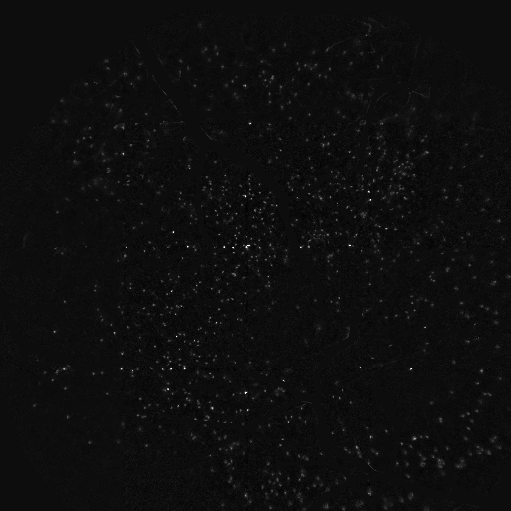
\includegraphics[width=\textwidth]{figs/composite_A.png}
      \caption*{A}
    \end{minipage}
    \begin{minipage}{0.49\textwidth}
      \centering
      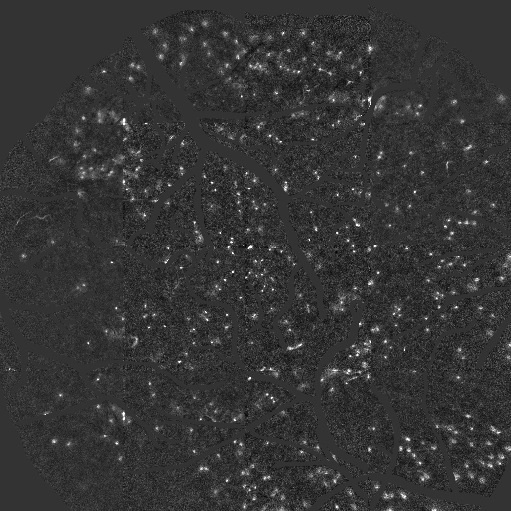
\includegraphics[width=\textwidth]{figs/composite_B.png}
      \caption*{B}
    \end{minipage}

    \begin{minipage}{0.49\textwidth}
      \centering
      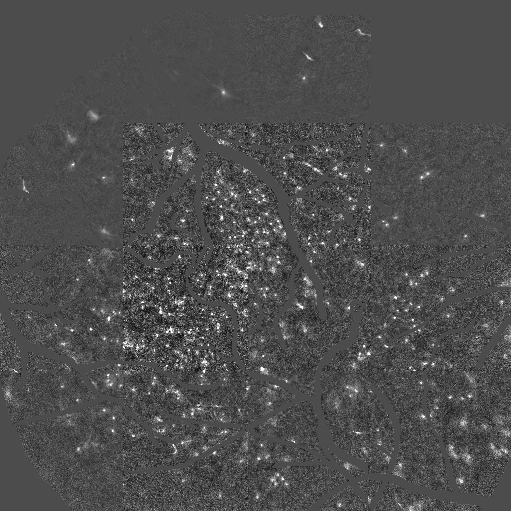
\includegraphics[width=\textwidth]{figs/composite_C.png}
      \caption*{C}
    \end{minipage}
    \begin{minipage}{0.49\textwidth}
      \centering
      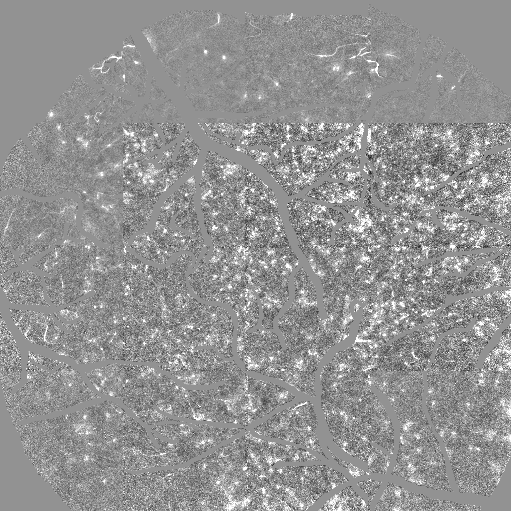
\includegraphics[width=\textwidth]{figs/composite_D.png}
      \caption*{D}
    \end{minipage}
    \caption{\footnotesize Aggregate images for each neuronal cluster. Clusters appear to correspond to the depth of the soma in which neurons are located. Cluster A is most in focus, cluster D is most out of focus.}
    \label{fig:clusterdepths}
\end{figure}

\begin{figure}[h]
    \centering

    \begin{minipage}{0.49\textwidth}
      \centering
      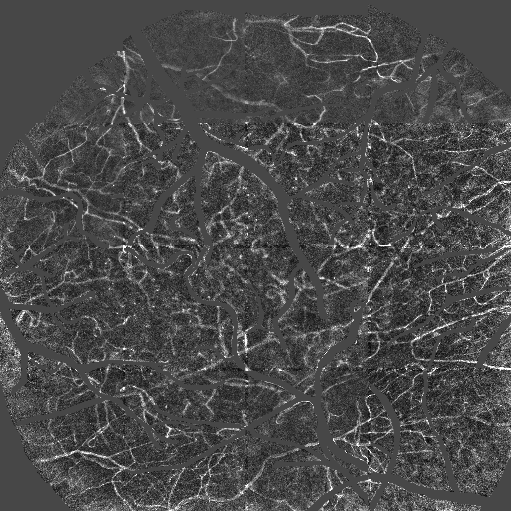
\includegraphics[width=\textwidth]{figs/vessels_DC.png}
      \caption*{High Intensity Vesseles}
    \end{minipage}
    \begin{minipage}{0.49\textwidth}
      \centering
      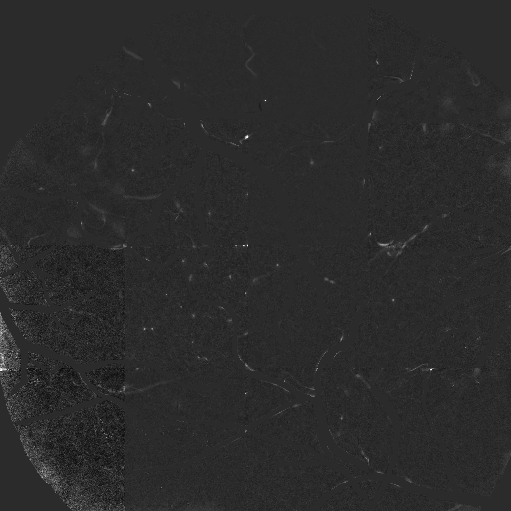
\includegraphics[width=\textwidth]{figs/remaining_vesseles.png}
      \caption*{Low Intensity Vesseles}
    \end{minipage}
    \caption{\footnotesize Aggregate images for background structure clusters. The high intensity structure lies in the region between clusters C and D in the dendrogram. The two clusters greatly differ in measured intensity.}
    \label{fig:clusterdepths}
\end{figure}

\end{document}